\clearpage

\section{Experimental Setup}
\label{cp6:procedures}



\gm{You need to provide the overall
design first. Hard to understand why
the tasks are as they are. More "Design' up-front.}


To determine how a tool embedding a semantic-based technique might impact task completion, we designed an experiment where participants attempted two programming
 using (or not) a tool that applies the \texttt{BERT} technique (Section~\ref{cp5:approach-bert})
 to  identify task-text relevant---highlighting  the text automatically identified  in the artifacts available in a task. 


The research questions for this experiment consider whether:



\begin{enumerate}
    \item \textit{a developer produce a more correct solution when assisted by such a tool;}
    \item \textit{the text automatically identified is similar to text that developers deem relevant to that task; and if}
    \item \textit{a developer finds that the text automatically identified and highlighted assisted them complete a particular task.}
\end{enumerate}



To investigate these research questions, 
we compare solutions where participants dit, or did not, have tool support by
running a set of test cases that evaluate the correctness of their submitted solutions.


In the tasks without tool support we asked participants to manually indicate the text that they deemed useful to their task.
We use the manually provided text to investigate to which extent our tool identifies the same text.


We complement this analysis by asking participants to indicate how useful were the highlights shown in each of the artifacts available in the tool-assisted task
and by requesting participants to provide any additional feedback that they wished to share about the tool or the experiment.






We detail experimental procedures in the following subsections.






% Our experiment's main hypothesis is that:


% \medskip
% \begin{bluequote}
%     \textit{text automatically identified by a semantic-based technique assists a 
%     developer complete her software development task.} 
% \end{bluequote}



% To test this hypothesis, 
 
%  \gm{Setting this up as a test of
%  a hypothesis sets a high bar where
%  there will be expectations of
%  refuting a null hypothesis. Is that
%  where you want to go?}

% %  For each of these tasks, we provided to the participants a curated list of natural language artifacts related to the task
% % and we asked them to code a solution for the task.
 
 
% %  when assisted (or not) by a
% %  tool that embeds one of the semantic-based techniques that we have explored previously ({Section~\ref{cp5:results-all}). 

% \gm{You need to provide the overall
% design first. Hard to understand why
% the tasks are as they are. More "Design' up-front.}

% In a first task, a participant manually identifies text relevant to that task (while performing the task)
% in a set of curated artifacts containing information that could assist the participant complete the task at hand.
% With this first task, we evaluate how the text that a participant manually identified as relevant
% compares to the text that an automatic technique would identify for that same task. 



% In a second task, each artifact associated to the task has a set of highlighted sentences. These 
% sentences represent text that an automatic approach ({Section~\ref{cp5:results-all}) identified as potentially useful for that task. 
% We ask a participant to indicate whether the highlights shown helped her complete their task.
% Hence, with this second task, we evaluate what is the participants' perceived usefulness of the text automatically identified.





% % \art{Add a figure to help summarizing the experimental setup?}



% \art{say somewhere that the experiment was performed remotely and without the researcher's assistance. }


\subsection{Design}


The experiment's independent variable represents the task configuration, i.e., if a participant had to manually indicated what text they deemed relevant to a task
or if our tool automatically did this step. We refer to these two configurations as \textit{manual} or \textit{tool-assisted}. 


Based on our independent variable, we follow a \textit{within-subjects} design. Each participant is exposed to exactly one manual task and one tool-assisted task.
We assigned tasks to a participant randomly. Nonetheless,  
we ensured that each task configuration (manual or tool-assisted) was seen by an equal number participants.
\gm{how is this design within-subjects?
Aren't you comparing across
the tasks which means across subjects?}








\subsection{Tasks}
\label{sec:experiment-tasks}



We expect the experiment to be executed offline, i.e., the experiment has self-contained instructions that allow a participant to perform their assigned tasks without any supervision.
\gm{Why not just say the participants
completed the tasks on their own time?}
This requires tasks that are easy to understand and perform in a single experimental session. At the same time, our main hypothesis requires tasks for which a developer will likely benefit from the use of additional information to complete.


These criteria lead us to select Python w3resource tasks\footnote{\url{https://www.w3resource.com/python-exercises/}}
that required usage of at least one module external to the Python core modules~\cite{thiselton2019}.
By using an external module, we aim to reduce the likelihood that a participant 
can provide a solution for a task without consulting any of the artifacts accompanying that task. 






Table~\ref{tbl:python-tasks-modules} details the tasks that we have selected. 
We chose these tasks due to how they focus on modules widely adopted both by open source systems and by private companies.
For example, the \texttt{NYTimes} task involves using a HTML parser, namely \texttt{BeautifulSoup},
which Reddit---a social news aggregator with approximately 430 million monthly users---uses 
to parse urls and identify images shown on its posts' headlines~\cite{bs4-reddit}. 
Similarly, the \texttt{Titanic} task encompasses using \texttt{Pandas}, a data analysis and manipulation module
used in many open source data science projects~\cite{ma2017, shrestha2020}.





\begin{table}
\centering
\caption{Python tasks}
\begin{footnotesize}
\rowcolors{2}{}{lightgray}
\begin{tabular}{ll}
\hline
\textbf{Task} & \textbf{Description}                                                                                         \\
\hline
\hline
%
\parbox[l][1cm][c]{1cm}{Practice task}       &
\parbox[l][1cm][c]{11cm}{Given three dictionaries representing address books,
you must write an algorithm using the Python core \texttt{dict} module to merge them.}    \\
\hline
%
Distances     &
\parbox[l][1.3cm][c]{11cm}{Given a string representing a rendezvou point and a list of suggested picnic addresses
    you must write an algorithm using the \texttt{geopy} module to find the  picnic address closest to the rendezvou point.} \\
%
NYTimes       &
\parbox[l][1cm][c]{11cm}{Given a string representing the url for NY Times Today's,
    write an algorithm using the \texttt{BeautifulSoup} and \texttt{requests} modules to scrape all the headlines of that page.}
\\
%
Titanic       &
\parbox[l][1cm][c]{11cm}{Given a string representing a url for the titanic dataset,
    you must write an algorithm using the \texttt{pandas} and \texttt{seaborn} modules to create a barchart of the data.}    \\
    
\hline
\end{tabular}
\end{footnotesize}
% \smallskip
\label{tbl:python-tasks-modules}
\end{table}









\subsection{Artifacts}
\label{sec:experiment-artifacts}


Each task requires a set of artifacts that a participant could peruse for information that could assist them complete the task.
We select artifacts for a task following procedures similar to the ones we used to create the \acs{DS-android} dataset (Chapter~\ref{ch:android-corpus}). 
For each of the tasks in Table~\ref{tbl:python-tasks-modules}, we use the Google search engine to obtain up to ten artifacts that likely contain relevant
information for that task. 






\subsection{Participants}



We advertised our study to both developers in our professional network and to computer science students at the several universities. 
This provides for breadth of experience where both novice and expert developers attempt the tasks in our experiment. 


With regards to computer science students, we sent the study only to third and fourth-year students to ensure that they had the necessary background required to perform the study's taks.
At this point in the curriculum, students should be familiar with Python and they should be able to come up with a solution 
for a software task when provided with artifacts containing information for that task.


To compensate participants for their time, we offered them the opportunity to enter a raffle for one of two iPads 64 GB.






\subsection{Procedures}
\label{cp6:evaluation-procedures}



The experiment was completely offline, i.e., it could be performed at a participant's personal computer
without the presence of one of the researchers. Each participant had to complete a practice task---separated from the experimental tasks---and two tasks (manual and tool-assisted) drawn from the tasks in Table~\ref{tbl:python-tasks-modules}. 


Each experimental session lasted no more than two hours; this length of time was selected based on two pilot sessions. 
Feedback from these pilots also helped to refine the experiment's instructions, where we included a short video showing how to install the web browser plugin and how to use Colab, the online environment where participants performed each task (Section~\ref{cp6:environment}).






We began each session gathering consent and requesting participants to install a web browser plugin which we used to gather data.
Setup was followed by a short tutorial explaining the experiment and describing how to use the plugin and Colab. 
The practice task allowed participants to familiarize themselves with the content of a task, the web browser plugin and Colab. 



For each task, including the practice tasks, we asked a participant to write a solution for the task
when provided with a fixed set of artifacts, e.g., official API documentation, Stack Overflow posts, or web tutorials, 
associated with that task.  


In the control task, a participant was instructed to use the web browser plugin to highlight any text that they deemed relevant to the task-at-hand. 
\gm{Do they highlight text as they
work or after the task?}
In the tool assisted task, the plugin automatically highlighted sentences that our semantic-based technique identified as relevant for the task. 
For this second task, we had one extra step asking the participant to rate---using a Likert scale---how helpful were the highlights automatically identified per artifact available. 
\gm{More detail about exactly
what participants were asked to
do and experimental materials
should be published or in Appendix
of thesis.}


We concluded the study by asking participants if they would like to provide any additional information and 
by giving them the opportunity to join the raffle, if so they wished. 



% \subsubsection{Summary of procedures}

% Based on our experimental procedures, we could gather:



% \begin{enumerate}
%     \item a participant's submitted solution (written Python code) for each task;
%     \item a participant's highlights for the control task; 
%     \item a participant's perception on the usefulness of the automatically identified highlights for the tool assisted task, and;
%     \item any additional feedback (written text) that a participant wished to provide us.
% \end{enumerate}




\subsection{Colab}
\label{cp6:environment}


To ensure that participants had the same conditions to perform each task
and also to minimize setup instructions, we used Google Colab\footnote{\url{https://colab.research.google.com/}} as our coding environment. 
% By using Colab, we also expect setup instructions to be minimal 
% so that we allow a participant to focus on the task and experimental procedures.



Figure~\ref{fig:nytimes-task-colab} shows an example of our online environment for the \texttt{NYTimes} task.
At the left-hand side, participants had the task description and examples of input and output scenarios as well as a list of resources associated with that task. 
By clicking on the coding environment link, participants were redirected to Colab (right-hand side),
where they had a code editor with amenities commonly found in modern IDEs, such as code completion and syntax highlighting. 



Through Colab, a participant could compile their solution and test it against the examples shown alongside the task description.
Upon testing, the system would display full details about the test cases, e.g., the test's input, which assertion failed, and why. 




\clearpage

\begin{landscape}
\begin{figure}
    \centering
    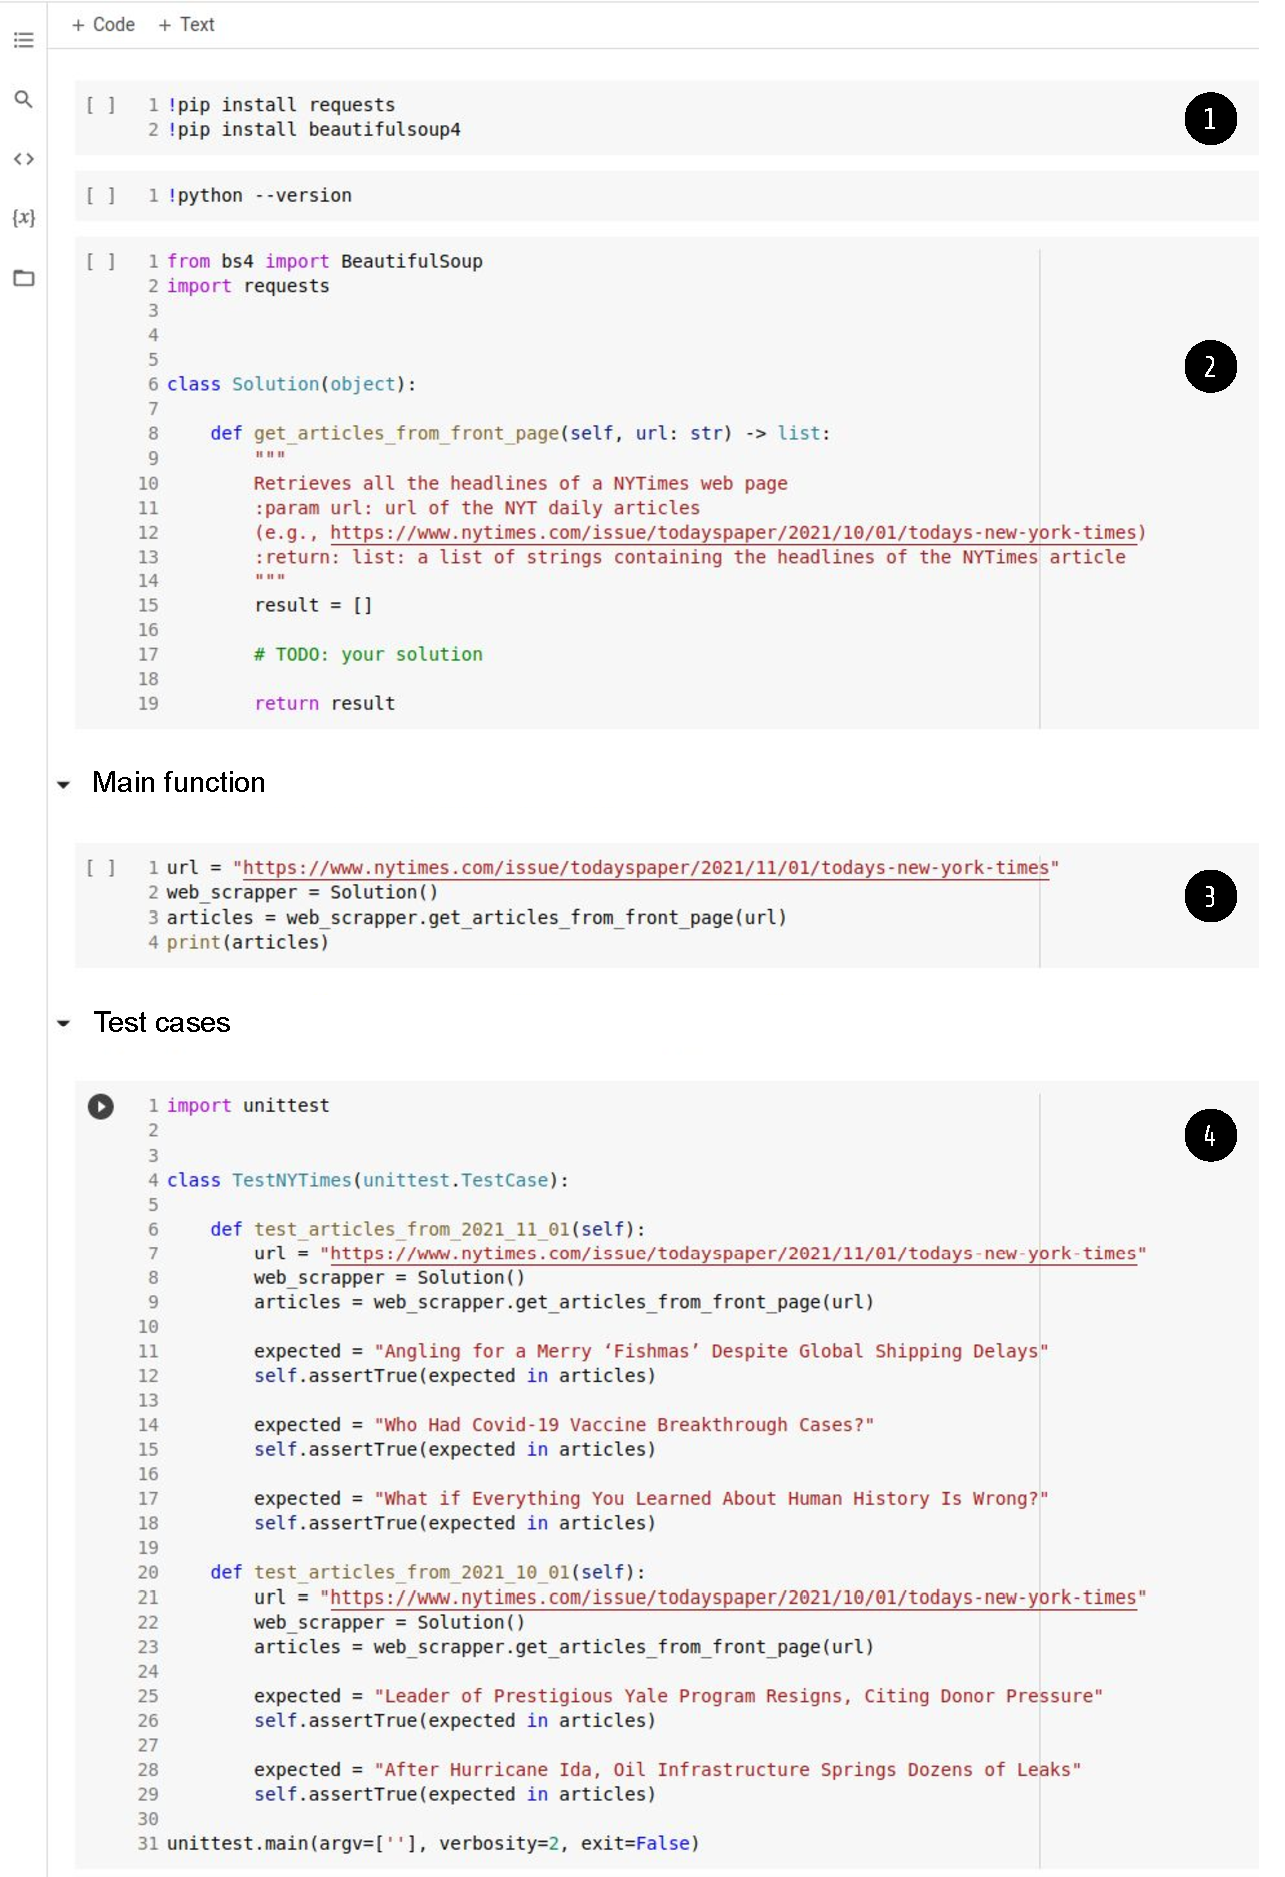
\includegraphics[width=1.5\textwidth]{cp6/task-colab.pdf}
    \caption{NYTimes task and Colab environment.}
    \label{fig:nytimes-task-colab}
\end{figure}
\end{landscape}

\clearpage


\subsection{Analysis}



Table~\ref{tbl:experiment-data} summarizes the data we collected based on experimental procedures.
We use the gathered data to investigate our main hypotheses according to the following metrics.



\begin{table}
\caption{Data collected}
\begin{small}
\vspace{-1mm}  


\begin{threeparttable}    
\rowcolors{2}{}{lightgray}
\begin{tabular}{ll}
\hline    
\textbf{} & \textbf{Data collected}  \\ 
\hline
\hline
1 & 
\parbox[l][0.8cm][c]{11cm}{
    participant's submitted solution (written Python code) for each task
}  
\\
%
2 & 
\parbox[l][0.8cm][c]{11cm}{
     participant's highlights for the control task
}  \\
3 & 
\parbox[l][1cm][c]{11cm}{
    a participant's perception on the usefulness of the automatically identified highlights for the tool assisted task
}  \\
4 & 
\parbox[l][0.8cm][c]{11cm}{
    any additional feedback (written text) that a participant wished to provide us
}  \\
\hline
\end{tabular}
\end{threeparttable}    
\end{small}
\smallskip
\label{tbl:experiment-data}
\end{table}
    



\subsubsection{Submitted Solution}

 
The correctness of a submitted solution is measured by the number of passing test cases
when running that solution against a set of 10 test cases. 
A solution with compile errors has a correctness score of zero.


\smallskip
\begin{small}


\begin{equation}
    Correctness = \frac{ \text{\textit{\# of passing test cases}}}{\text{\textit{\#  of test cases}}}
\end{equation}
\end{small}

% \smallskip
% According to this definition, 


\subsubsection{Manual Highlights}


We compare the participants' manual highlights  against the ones automatically identified by our semantic-based technique. 
For that, we use \textit{precision} and \textit{recall} metrics. 




Precision measures the fraction of the automatically identified text that was  considered relevant
by the participants.

\smallskip
\begin{small}


\begin{equation}
    Precision = \frac{
        \text{\textit{automatic highlights}~} \cap 
        \text{~\textit{manual highlights}}
    }{\text{\textit{automatic highlights}}}
\end{equation}
\end{small}


Recall represents how many of all the manual highlights were identified by the semantic-based technique that we applied.

\smallskip
\begin{small}

\begin{equation}
    Recall = \frac{
        \text{\textit{automatic highlights}~} \cap 
        \text{~\textit{manual highlights}}
    }{\text{\textit{manual highlights}}}
\end{equation}
\end{small}

\medskip
\art{Argue which metric matters the most here}


\art{Discuss how to account for variability in what the participants highlighted}



\subsubsection{Usefullness of the Automatic Highlights}


We use a diverging stacked bar chart~\cite{Heiberger2014} to analyze the  Likert scale
responses on the usefulness of the text automatically identified.


Usefulness indicates the percentage of responses agreeing or disagreeing with whether sentences
automatically highlighted assisted a participant in completing a task.


\smallskip
\begin{small}

\begin{equation}
Usefullness = \frac{
    \text{\textit{\# of responses at i}}
}{
    \text{\textit{total \# of responses}}
}
\end{equation}
        

\begin{equation*}
i \in \{ 
    \text{\textit{
        (strongly) agree, neither agree or disagree, (strongly) disagree
    }}  
\}
\end{equation*}
\end{small}

% This analysis complements the quantitative comparison of manual and automatic highlights.
% By asking participants to reflect on the usefulness of the text automatically identified, 
% we seek to minimize risks related to how a participant might have missed highlighting
% text that assisted them complete a task~\cite{easterbrook2008}.





\subsubsection{Written Feedback}

 
We use qualitative methods to analyze participants' responses to the open-ended questions. 

\art{Think this through...}




\clearpage

